% Persistent Soft-Plan Decoding -- repository technical report
% Build: latexmk -pdf -interaction=nonstopmode -halt-on-error Persistent_Soft_Plan_Block_Proposal_Technical_Report.tex
% Version 0.1, 2026-10-14. Requires an ordinary TeX Live distribution.
\documentclass[11pt,letterpaper]{article}
\usepackage[T1]{fontenc}
\usepackage[utf8]{inputenc}
\usepackage{lmodern}
\usepackage{microtype}
\usepackage[margin=0.91in,headheight=17pt]{geometry}
\usepackage{amsmath,amssymb,amsfonts,mathtools}
\usepackage{booktabs,array,tabularx,multirow,longtable}
\usepackage{graphicx,float}
\usepackage{tikz}
\usetikzlibrary{arrows.meta,positioning,calc,fit,matrix,backgrounds}
\usepackage{pgfplots}
\pgfplotsset{compat=1.18}
\usepackage{xcolor}
\usepackage{hyperref}
\usepackage{cleveref}
\usepackage{fancyhdr}
\usepackage{enumitem}
\usepackage{listings}
\usepackage{caption}
\usepackage{titlesec}
\usepackage{needspace}
\usepackage{etoolbox}
\definecolor{navy}{HTML}{172A43}
\definecolor{bluegray}{HTML}{50647D}
\definecolor{teal}{HTML}{007C83}
\definecolor{orange}{HTML}{B46415}
\definecolor{green}{HTML}{2E7656}
\definecolor{muted}{HTML}{EEF3F7}
\definecolor{warm}{HTML}{FCF4E9}
\definecolor{linegray}{HTML}{D9E1E8}
\definecolor{ink}{HTML}{253545}
\hypersetup{colorlinks=true,linkcolor=navy,urlcolor=teal,citecolor=teal,pdftitle={Persistent Soft-Plan Decoding: Technical Report},pdfauthor={Lucka Barbeau}}
\titleformat{\section}{\Large\bfseries\color{navy}}{\thesection}{0.65em}{}
\titleformat{\subsection}{\large\bfseries\color{navy}}{\thesubsection}{0.65em}{}
\titleformat{\subsubsection}{\normalsize\bfseries\color{teal}}{\thesubsubsection}{0.65em}{}
\titlespacing*{\section}{0pt}{2.2ex plus 0.3ex minus .2ex}{0.8ex}
\titlespacing*{\subsection}{0pt}{1.65ex plus 0.3ex minus .2ex}{0.6ex}
\captionsetup{font=small,labelfont={bf,color=navy},skip=6pt}
\setlist[itemize]{nosep,topsep=4pt,leftmargin=18pt}
\setlist[enumerate]{nosep,topsep=4pt,leftmargin=20pt}
\pagestyle{fancy}
\fancyhf{}
\fancyhead[L]{\small\color{bluegray}MYLOCAL\_LLM / ARCHITECTURE NOTE 0080}
\fancyhead[R]{\small\color{bluegray}14 OCT 2026 \quad v0.1}
\fancyfoot[L]{\small\color{bluegray}Working technical report -- not peer reviewed}
\fancyfoot[R]{\small\color{bluegray}\thepage}
\renewcommand{\headrulewidth}{0.35pt}
\renewcommand{\footrulewidth}{0pt}
\newcommand{\plan}{\textsc{Plan}}
\newcommand{\dec}{\textsc{Dec}}
\newcommand{\CE}{\operatorname{CE}}
\newcommand{\softmax}{\operatorname{softmax}}
\newcommand{\R}{\mathbb{R}}
\newcommand{\projecturl}{\url{https://github.com/Luckabarbeau/MyLocal_LLM}}
\newcommand{\term}[1]{\textbf{#1}}
\newcommand{\code}[1]{\texttt{#1}}
\newcommand{\note}[1]{\par\noindent\colorbox{muted}{\parbox{\dimexpr\linewidth-2\fboxsep\relax}{\small #1}}\par}
\lstset{basicstyle=\ttfamily\footnotesize,keywordstyle=\color{teal},commentstyle=\color{bluegray},stringstyle=\color{orange},breaklines=true,columns=fullflexible,keepspaces=true,frame=single,framerule=0.4pt,rulecolor=\color{linegray},xleftmargin=3pt,xrightmargin=3pt,aboveskip=7pt,belowskip=7pt,showstringspaces=false}
\begin{document}
\begin{center}
  {\fontsize{22}{27}\selectfont\bfseries\color{navy}Persistent Soft-Plan Decoding}\par\vspace{4pt}
  {\Large\color{bluegray}A Block-Causal Probabilistic Proposal Architecture\\for Language Modeling}\par\vspace{13pt}
  {\large Lucka Barbeau}\par\vspace{3pt}
  {\small MyLocal\_LLM research project \;\textbullet\; \projecturl}\par\vspace{8pt}
  {\color{teal}\rule{0.75\linewidth}{1.0pt}}\par\vspace{6pt}
  {\small \textbf{Technical report v0.1} \quad 14 October 2026 \quad Experimental architecture series 0080}\par
\end{center}
\vspace{4pt}
\noindent\colorbox{muted}{\parbox{\dimexpr\linewidth-2\fboxsep\relax}{\vspace{5pt}\small\textbf{Status.} This is a dated, reproducibility-oriented project research note, not a peer-reviewed paper or a state-of-the-art claim. Results below are from local 7M-class CPU experiments reported through 2,500 additional expanded-corpus training steps. The separate approximately 500M-parameter integration is \emph{not} evaluated here for quality or production throughput.\vspace{5pt}}}

\begin{abstract}
We describe a block-causal language-model architecture that predicts a fixed group of $K$ future-token distributions from one causal Transformer boundary state, converts all $K$ distributions into differentiable soft token embeddings, and supplies them as a \emph{persistent bidirectional plan prefix} to a lightweight causal decoder. The decoder selects tokens sequentially, conditioning on both the original soft plans and the tokens already committed within the block. A residual correction to the backbone's shared vocabulary logits yields normalized next-token distributions; joint supervision trains both direct future proposals and corrected predictions. The architecture represents a tractable factorization of a conditional $K$-token distribution without constructing an explicit $V^K$ joint vocabulary.

Preliminary experiments on a roughly 7M-class model ($K=4$, 2,048-token vocabulary) show improving held-out cross-entropy on expanded training data, measurable reliance on cross-position soft-plan inputs, and particularly pronounced sensitivity to future-position plans at the first output position. At step 2,500, full-plan cross-entropy is 4.1840 nats/token; neutralizing all future plans for the first target increases its loss by 0.2908 nats/token. These are \emph{frozen-model interventions}, not causal estimates of an independently retrained architecture's advantage. A commitment-stride comparison on 256 reference tokens favors preserving the four-token plan ($S=4$: 3.96349 nats/token) over replanning every one or two tokens ($S=1$: 4.02431, $S=2$: 4.02332), while free-running generation remains markedly incoherent. We outline precise limitations, code-level reproduction, and next experiments required to test planning, generalization, scaling, and performance.
\end{abstract}
\clearpage
\tableofcontents
\clearpage

\section{Motivation, scope, and hypotheses}
Conventional autoregressive (AR) language modeling uses a causal representation $h_t=f_\theta(x_{\leq t})$ to predict one next-token distribution. A sequence of future tokens is generated by repeating this operation after each commitment. The present work explores a different allocation of computation: the expensive causal backbone first describes several plausible next positions, while a much smaller module learns how those uncertain predictions should be reconciled into a valid sequence.

The initial intuition is illustrated by the hypothetical phrase pair \emph{New York} versus \emph{San Francisco}: a plausible first token constrains the next one, but an uncertain next-token distribution might benefit from representations of possible later continuations. The architecture does not enumerate such phrases or create an explicit compound tokenizer. Instead, it gives a learned causal decoder access to all projected soft future marginals, including those corresponding to already committed positions.

The central research questions are:
\begin{enumerate}
\item Can the decoder use \emph{future-position proposal representations} to improve earlier token probabilities while remaining strictly causal with respect to ground-truth targets?
\item Can the original soft proposals remain useful \emph{after} the corresponding token has been committed, providing information complementary to the hard token embedding?
\item Does the mechanism improve free-running coherence, repetition behavior, likelihood, or efficiency relative to carefully matched AR and multi-token baselines?
\item How does the optimal proposal horizon $K$, commitment stride $S$, and decoder capacity change as the backbone grows?
\end{enumerate}
These are hypotheses. The early measurements support a dependence on soft-plan representations; they do not yet prove higher-level semantic planning or superiority to matched AR systems.

\subsection{Relation to existing work}
The design is related to, but distinct from, several existing approaches. Multi-token prediction supervises multiple future horizons above a shared backbone \cite{gloeckle2024}; multiple decoding heads also appear in speculative or tree-based acceleration systems such as Medusa \cite{cai2024}. Prefix and seq2seq attention masks that combine bidirectional context with causal generation have precedents, including UniLM \cite{dong2019}. Standard Transformers provide the underlying self-attention mechanism \cite{vaswani2017}. This work focuses on the particular \emph{combination} of full soft future distributions, an explicitly bidirectional small PLAN prefix, a separate hard committed-token stream, persistent access to both throughout a block, and end-to-end corrected-token training. This description should not be treated as a comprehensive prior-art or patent-novelty assessment.

\section{Architecture and causal information flow}
\subsection{Sequence alignment and proposal boundaries}
Let $x_{\leq t}$ denote the genuinely available context immediately before generation of token $y_1$. In the implemented training alignment, the ordinary source tokens are paired with their conventional shifted next-token labels; the backbone's proposal boundary for a block begins at the hidden state that has already processed the source token immediately preceding that block. In a training window, all source positions can be processed in a single causal trunk pass, but the proposal for a given block is formed \emph{only} from that block's corresponding boundary state. Thus no target $y_j$ from the proposed block is used to construct the plan.

For a proposal horizon $K$, one boundary state $h\in\R^d$ produces
\begin{equation}
  L=[\ell_1,\ldots,\ell_K]\in\R^{K\times V}, \qquad
  p_j=\softmax(\ell_j)\in\Delta^{V-1},
  \label{eq:proposals}
\end{equation}
where $V$ is the vocabulary size. These $p_j$ are \emph{marginal horizon proposals conditioned on the same pre-block context}, not independently sampled tokens, and not an explicit joint probability table.

\subsection{Shared multi-horizon proposal head}
The implementation uses one shared nonlinear head and the backbone's existing (untied) vocabulary output projection $W_{\mathrm{vocab}}$. Writing $a_j$ for a learned horizon embedding, the implemented form is
\begin{align}
  u_1 &= h, \\
  u_j &= h+\rho\,\tanh(hW_{\mathrm{ctx}}+a_j)W_{\mathrm{back}},\quad j=2,\ldots,K,\\
  \ell_j &= W_{\mathrm{vocab}}(u_j),
  \label{eq:head}
\end{align}
with compatible tensor orientation understood. In the default research implementation, $\rho=0.1$. Horizon one uses the same normalized boundary hidden state and vocabulary projection as a conventional one-step LM head. Later horizons share the small proposal MLP and the same vocabulary projection; there are no $K$ independent vocabulary matrices.

\subsection{Differentiable probability-derived PLAN embeddings}
The entire proposal distribution enters the small decoder through an expectation over the original input embedding table $E\in\R^{V\times d}$:
\begin{equation}
  z_j=p_j^\top E =\sum_{v=1}^{V}p_j(v)E_v\in\R^{d}.
  \label{eq:expectation}
\end{equation}
This is a \emph{compressed soft representation}. The decoder does \emph{not} directly receive the complete $V$ probabilities as a sequence of $V$ inputs, and $z_j$ need not preserve every detail of $p_j$ because $d\ll V$. Gradients nevertheless flow through the expectation and the proposal softmax to the proposal logits, as well as into the input embeddings.

With learned projections $W_P,W_D$ and learned position vectors $r^P_j,r^D_j$, the two streams are
\begin{align}
  P_j &= W_Pz_j+r^P_j,\quad j=1,\ldots,K,\\
  D_1 &= b_{\mathrm{BOS}}+r^D_1,\\
  D_j &= W_DE[y_{j-1}]+r^D_j,\quad j=2,\ldots,K.
  \label{eq:streams}
\end{align}
The distinction is essential: \emph{$P_{j-1}$ is never replaced by $E[y_{j-1}]$ after commitment}. The original predicted representation remains present in the PLAN stream, while the actual preceding token enters a separate DEC position. The PLAN and DEC embeddings use different learned input projections even though they refer to the same underlying input embedding table.

\begin{figure}[t]
\centering
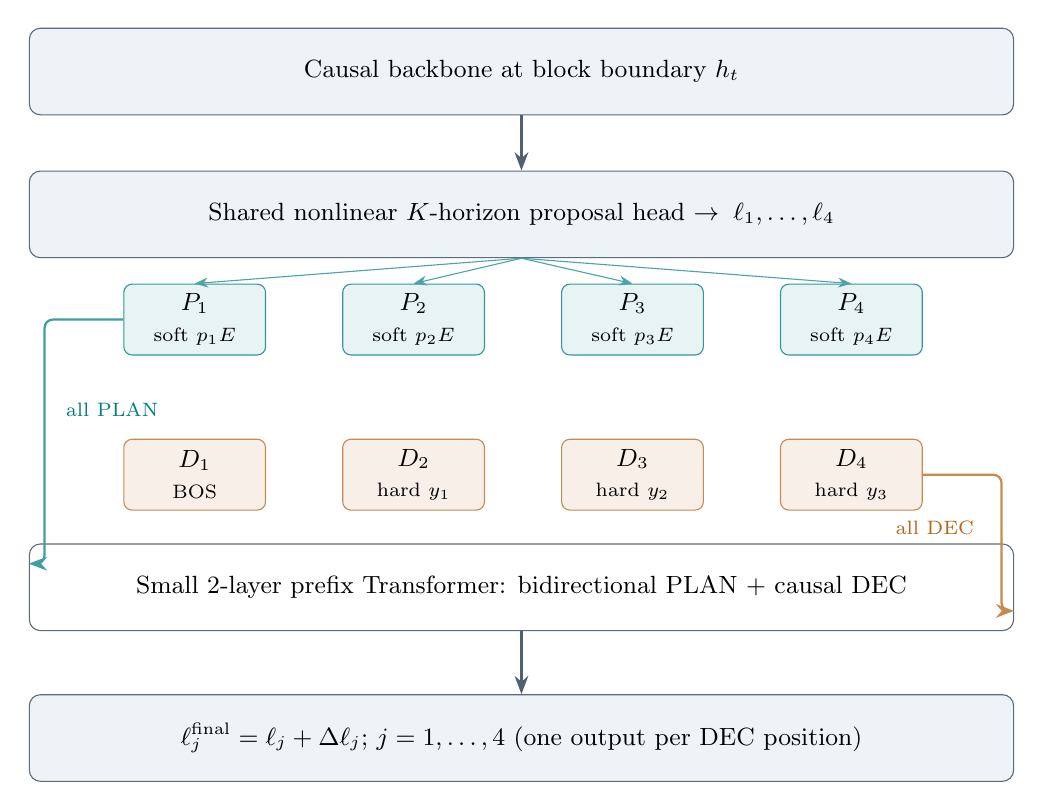
\begin{tikzpicture}[font=\small, node distance=7mm, >=Stealth,
  main/.style={draw=navy!70,fill=muted,rounded corners=4pt,minimum height=11mm,align=center},
  plan/.style={draw=teal!80,fill=teal!9,rounded corners=3pt,minimum height=9mm,minimum width=18mm,align=center},
  dec/.style={draw=orange!75,fill=orange!10,rounded corners=3pt,minimum height=9mm,minimum width=18mm,align=center}]
\node[main,minimum width=125mm] (back) {Causal backbone at block boundary $h_t$};
\node[main,below=of back,minimum width=125mm] (proposal) {Shared nonlinear $K$-horizon proposal head $\to\; \ell_1,\ldots,\ell_4$};
\foreach \j in {1,...,4} {
  \node[plan] (p\j) at ({-4.15+2.78*(\j-1)},-3.15) {$P_{\j}$\\\scriptsize soft $p_{\j}E$};
  \pgfmathtruncatemacro{\prev}{\j-1}
  \node[dec] (d\j) at ({-4.15+2.78*(\j-1)},-5.12) {\ifnum\j=1 $D_1$\\\scriptsize BOS\else $D_{\j}$\\\scriptsize hard $y_{\prev}$\fi};
}
\draw[->,navy!75,thick] (back)--(proposal);
\foreach \j in {1,...,4} {\draw[->,teal!70] (proposal.south) -- (p\j.north);}
\node[main,fill=white,minimum width=125mm] (prefix) at (0,-6.55) {Small 2-layer prefix Transformer: bidirectional PLAN + causal DEC};
% Route the two streams around the other row for legibility.
\draw[->,teal!75,thick,rounded corners=3pt] (p1.west) -- ++(-1.0,0) |- ([yshift=3mm]prefix.west);
\draw[->,orange!75,thick,rounded corners=3pt] (d4.east) -- ++(1.0,0) |- ([yshift=-3mm]prefix.east);
\node[font=\scriptsize,teal] at (-5.2,-4.3) {all PLAN};
\node[font=\scriptsize,orange] at (5.25,-5.8) {all DEC};
\node[main,below=8mm of prefix,minimum width=125mm] (out) {$\ell_j^{\mathrm{final}}=\ell_j+\Delta\ell_j$; $j=1,\ldots,4$ (one output per DEC position)};
\draw[->,navy!75,thick] (prefix)--(out);
\end{tikzpicture}
\caption{The implemented $K=4$ layout. The full PLAN remains accessible during all four sequential token commitments. The diagram separates the soft plan from the shifted hard-token stream; arrows from all PLAN and DEC positions into the small decoder indicate allowed pathways, not equal attention weights.}
\label{fig:architecture}
\end{figure}

\subsection{A 2K-position prefix Transformer}
The small decoder concatenates all PLAN positions \emph{before} all DEC positions:
\begin{equation}
  X_{\mathrm{small}}=[P_1,\ldots,P_K,D_1,\ldots,D_K]\in\R^{2K\times d_D}.
\end{equation}
Its attention mask $A\in\{0,1\}^{2K\times2K}$ is specified by
\begin{equation}
  A_{qk}=\begin{cases}
    1,&q\leq K,\;k\leq K,\\
    1,&q>K,\;k\leq K,\\
    1,&q>K,\;K<k\leq q,\\
    0,&\text{otherwise.}
  \end{cases}
  \label{eq:mask}
\end{equation}
The first $K$ rows are fully bidirectional over the \emph{predicted} PLAN positions and cannot read any DEC row. Every DEC row can read all PLAN positions and only its own or earlier DEC rows. The graph is block-causal because no PLAN input depends on a true token in the proposed block; all DEC inputs are shifted committed tokens.

\begin{figure}[ht]
\centering
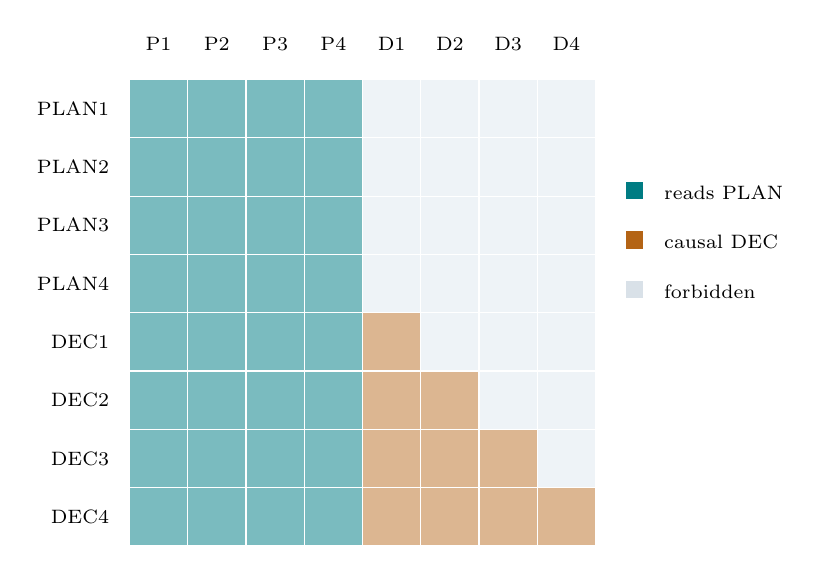
\begin{tikzpicture}[x=0.74cm,y=0.74cm,font=\scriptsize]
\foreach \i in {1,...,8}{
 \pgfmathtruncatemacro{\prev}{\i-4}
 \node[anchor=east] at (-0.18,8.5-\i) {\ifnum\i<5 PLAN\i\else DEC\prev\fi};
 \node at (\i-0.5,8.62) {\ifnum\i<5 P\i\else D\prev\fi};
}
\foreach \i in {1,...,8}{\foreach \j in {1,...,8}{
  \ifnum\i<5
    \ifnum\j<5 \def\cellcol{teal!52}\else \def\cellcol{muted}\fi
  \else
    \ifnum\j<5 \def\cellcol{teal!52}\else
       \ifnum\j>\i \def\cellcol{muted}\else \def\cellcol{orange!47}\fi
    \fi
  \fi
  \fill[\cellcol,draw=white] (\j-1,8-\i) rectangle (\j,9-\i);
}}
\node[anchor=west] at (8.35,6.1) {\textcolor{teal}{\rule{0.22cm}{0.22cm}} \; reads PLAN};
\node[anchor=west] at (8.35,5.25) {\textcolor{orange}{\rule{0.22cm}{0.22cm}} \; causal DEC};
\node[anchor=west] at (8.35,4.4) {\textcolor{linegray}{\rule{0.22cm}{0.22cm}} \; forbidden};
\end{tikzpicture}
\caption{Exact attention permission structure for $K=4$. Rows are queries and columns are keys. The forbidden PLAN$\leftarrow$DEC region prevents targets from leaking into soft proposals through decoder self-attention.}
\label{fig:mask}
\end{figure}

The small stack uses dense self-attention with RMSNorm and SwiGLU feed-forward layers; the tested CPU decoder has two layers, width 128 and four attention heads, with no MoE inside the decoder. During teacher-forced training all DEC outputs are evaluated in one masked forward per bounded group of independent blocks. In cached inference, the PLAN prefix is processed once, its per-layer keys/values are retained, and each committed-token DEC position is appended sequentially.

\subsection{Residual output and conditional block factorization}
The small decoder outputs a position-specific correction $\Delta\ell_j$, using a projection back to the backbone's hidden width and the \emph{same} vocabulary output projection as the proposal head:
\begin{equation}
  \ell_j^{\mathrm{final}}=\ell_j+\Delta\ell_j,\qquad
  q_j(\cdot\mid c,y_{<j})=\softmax(\ell_j^{\mathrm{final}}).
  \label{eq:final}
\end{equation}
A valid conditional probability for a complete block is then defined autoregressively by
\begin{equation}
 Q_\Theta(y_{1:K}\mid c)=\prod_{j=1}^{K}q_j(y_j\mid c,y_{<j},Z(c)),
 \qquad Z(c)=(z_1,\ldots,z_K).
 \label{eq:joint}
\end{equation}
This \emph{implicit} joint sequence distribution is normalized without enumerating $V^K$ combinations. It is not a learned explicit categorical distribution over $V^K$ phrases. Because $Z(c)$ is computed from context alone, an unrestricted Bayes-optimal AR predictor conditioning on the same $c$ cannot gain additional information from $Z(c)$; the potential benefit is \emph{finite-model representation, optimization, or computation efficiency}.

\section{Training objective and implementation contracts}
\subsection{Joint loss and gradient paths}
Let $m_{bj}\in\{0,1\}$ indicate that horizon $j$ in block $b$ corresponds to a real supervised token, and let $N_{\rm valid}=\sum_{b,j}m_{bj}$. The actual objective is
\begin{align}
 \mathcal{L}_{\mathrm{final}}&=-\frac{1}{N_{\rm valid}}\sum_{b,j}m_{bj}\log q_{bj}(y_{bj}),\\
 \mathcal{L}_{\mathrm{proposal}}&=-\frac{1}{N_{\rm valid}}\sum_{b,j}m_{bj}\log p_{bj}(y_{bj}),\\
 \mathcal{L}&=\mathcal{L}_{\mathrm{final}}+\lambda\mathcal{L}_{\mathrm{proposal}},\qquad \lambda=0.5\text{ in the reported CPU experiment}.
 \label{eq:loss}
\end{align}
Each real token counts \emph{once} in the normalization; the two losses are not counted as two independent supervised examples. The final CE propagates gradients through the direct residual logits, the decoder, soft expectations $pE$, the proposal softmax, the shared embedding table, and the main causal boundary state. The auxiliary proposal CE provides direct training pressure at all horizons. An implementation with hand-written backward passes preserves both gradient routes.

\subsection{Causal safety and block scheduling}
Training enforces the following invariants:
\begin{itemize}
 \item A block's proposals read only its \emph{pre-block} causal boundary hidden state, never a later hidden state from the teacher-forced source window.
 \item PLAN positions cannot read DEC positions; DEC$_j$ sees only BOS, earlier real target tokens, and all precomputed PLAN positions.
 \item Document boundaries, end-of-sequence handling, routed-prefix history starts, and invalid tail masks are preserved; unrelated documents are not silently concatenated as one proposal block.
 \item Main-model routed memory is selected using a strictly pre-window query. The original local, dilated, sparse, and learned retrieval heads remain in the main backbone.
 \item The main trunk is run once per training window. The bounded $K$-block groups reuse gathered causal boundary states, accumulate gradient contributions there, and perform one main-trunk backward pass.
\end{itemize}
These invariants distinguish the architecture from merely providing the decoder with the future teacher-forced sequence. Inference additionally updates the main causal KV state \emph{only with committed tokens}, never provisional future predictions.

\subsection{Parameter and computational considerations}
The $K$ proposal logits are full-vocabulary distributions but reuse the backbone output projection, so the proposal head does not instantiate $K$ independent matrices of shape $d\times V$. The small decoder processes $2K$ positions, typically much shorter than the full active context. However, projecting and retaining all $K$ full-vocabulary logits, evaluating probability expectations, and differentiating through two CE objectives can still incur significant bandwidth, memory, and synchronization overhead. Exact GPU throughput, allocation peaks, and parity must be measured: a \emph{single trunk pass in training} does not automatically imply faster end-to-end inference or training than a matched standard AR model.

\section{Exploratory experimental setup}
\subsection{Two successive dataset regimes}
The CPU research experiment started with a compact two-source packed mixture, built using a preprocessing cap of 256 documents per source and an unchanged custom 2,048-token tokenizer. That restricted preparation contained only about 683,000 packed training tokens. The original $K=4$ CPU run trained for 5,000 steps on this smaller preparation. It was subsequently \emph{weight-only warm-started} on a separately prepared, much larger mixture capped at 50,000 documents per source, with a fresh AdamW optimizer state and sampling sequence. The larger dataset and held-out draw use distinct provenance; cross-dataset CE comparisons must therefore \emph{not} be interpreted as matched validation learning curves.

The two sources used for these experiments are named \code{fine\_edu} and \code{cosmopedia\_v2}. Packing, document/EOS boundaries, tokenizer fingerprint, mixture manifest, validation sample digests, sampler metadata and source-checkpoint lineage are recorded or checked by the current research pipeline. Expanded-run step numbers begin at \emph{zero} after the weight-only warm start and must not be confused with the original 5,000 optimizer steps.

\begin{table}[ht]
\centering\small
\caption{Reported experimental configuration for the expanded-corpus CPU checkpoint series. ``Approximately 7M'' is a model class, not an independently audited parameter count for this report.}
\label{tab:config}
\begin{tabularx}{\linewidth}{@{}lXlX@{}}\toprule
Backbone & 6 layers; width 192; MoE with 4 experts, top 2 & Attention & local, dilated, sparse, retrieval\\
Context & 256-token main memory horizon; 64-token targets & Vocabulary & 2,048 tokens\\
Proposals & $K=4$; shared head width 96; $\rho=0.1$ & Decoder & 2 layers; width 128; 4 heads\\
Objective & $\mathcal L_{\rm final}+0.5\mathcal L_{\rm prop}$ & Data & two-source packed mixture, expanded cap 50k/source\\
Optimizer & AdamW; fresh state at warm start & LR & $1\times10^{-4}$ in expanded run\\
Batching & batch 16; accumulation 1; block group 2 & Validation & 16 deterministic batches of 16 rows\\
Execution & NumPy CPU, float32 & Checkpoints & every 500 expanded steps\\
\bottomrule\end{tabularx}
\end{table}

The primary \emph{teacher-forced frozen-plan} validation uses the same fixed examples for each intervention: 16 batches of 16 rows, with up to 64 target tokens per row (at most 16,384 nominal token positions; the actual valid-token count can be smaller). The separate stride experiment intentionally uses only eight rows with up to 32 tokens each, totaling 256 scored tokens in the reported run.

\subsection{Measurements and terminology}
All CE values are negative log-likelihood in \emph{nats per real target token}; lower is better. ``Proposal CE'' scores $p_j$ against the true token at that horizon. ``Final CE'' scores $q_j$ using teacher-forced correct earlier tokens unless explicitly identified as \emph{causal-inference scoring}. The ``decoder gain'' is proposal CE minus final CE; it is not an independent information measure because the final model receives the correct earlier target tokens. ``Frozen masking gain'' means a change in final CE when some PLAN vectors are neutralized, without retraining model weights.

\section{Preliminary empirical results}
\subsection{Improving held-out final likelihood on expanded data}
\begin{table}[ht]
\centering
\caption{Reported expanded-corpus checkpoints, with the same held-out research-validation regime. The step-1,500 number is the mean of the four reported per-horizon validation CEs. Other values are from the frozen 0080K all-plan condition.}
\label{tab:curve}
\begin{tabular}{@{}rcc@{}}\toprule
Expanded optimizer step & Final CE (nats/token) & Status \\ \midrule
1,000 & 4.2909 & Fixed all-plan evaluation\\
1,500 & $\approx 4.2443$ & Reported horizon means\\
2,000 & 4.2101 & Fixed all-plan evaluation\\
2,500 & \textbf{4.1840} & Fixed all-plan evaluation\\
\bottomrule\end{tabular}
\end{table}

\begin{figure}[ht]
\centering
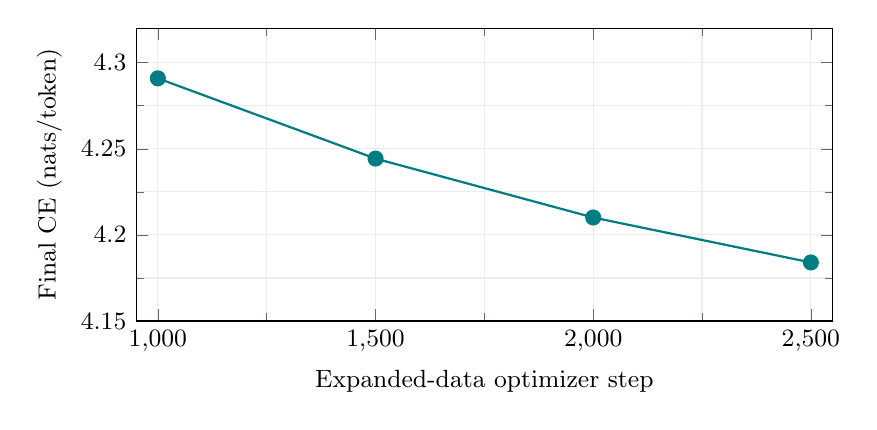
\begin{tikzpicture}
\begin{axis}[width=0.86\linewidth,height=5.3cm,xmin=950,xmax=2550,ymin=4.15,ymax=4.32,
 xlabel={Expanded-data optimizer step},ylabel={Final CE (nats/token)},
 xtick={1000,1500,2000,2500},grid=both,minor tick num=1,
 grid style={linegray!55},tick style={navy!70},label style={font=\small},tick label style={font=\small}]
\addplot[teal,thick,mark=*,mark size=2.5pt] coordinates {(1000,4.2909)(1500,4.2443)(2000,4.2101)(2500,4.1840)};
\end{axis}
\end{tikzpicture}
\caption{Held-out token likelihood continues improving after the weight-only warm start. This plot does not compare against a matched AR baseline.}
\label{fig:cecurve}
\end{figure}

At expanded step 2,000, the raw proposal and final losses by horizon show how much the sequential decoder changes the predictions:
\begin{table}[ht]
\centering
\caption{Expanded step-2,000 per-horizon teacher-forced validation. The proposal head sees the same pre-block context for all four positions; the decoder uses the real prior tokens for later positions.}
\label{tab:horizon}
\begin{tabular}{@{}lrrr@{}}\toprule
Horizon & Proposal CE & Final CE & Decoder gain\\\midrule
P1 & 4.7710 & 4.2271 & +0.5439\\
P2 & 5.8867 & 4.2035 & +1.6832\\
P3 & 6.2546 & 4.1931 & +2.0615\\
P4 & 6.4074 & 4.2167 & +2.1907\\\bottomrule
\end{tabular}
\end{table}
The final-position losses are nearly flat, while later direct proposals become progressively less certain. The natural explanation includes the true earlier tokens made available by teacher forcing; the table alone does not demonstrate multi-token reasoning or better free-running generation.

\subsection{What the frozen cross-position ablations actually change}
For each target horizon $j$, the 0080K evaluator holds fixed the main model, proposal logits and their additive residual-prior contribution, the source context, and the shifted \emph{true} committed-token prefix. Only the \emph{soft PLAN representations} are selectively replaced by a uniform-vocabulary expected embedding (with positional embeddings still present). The conditions are:
\begin{itemize}
\item \textbf{All:} $P_1,\ldots,P_K$ intact.
\item \textbf{Own only:} retain only $P_j$; neutralize all other PLAN vectors.
\item \textbf{Past + current:} retain $P_1,\ldots,P_j$; neutralize $P_{j+1},\ldots,P_K$.
\item \textbf{All except current:} retain every $P_i$ except $P_j$.
\item \textbf{Neutral:} neutralize all soft PLAN vectors while leaving direct logits and true shifted DEC inputs fixed.
\end{itemize}
The ablation loss penalty is $\Delta\CE_A=\CE_A-\CE_{\mathrm{all}}$. A positive penalty shows that the \emph{trained frozen predictor} is sensitive to that PLAN pathway. It is not a valid decomposition of mutual information, and masking can introduce out-of-distribution representations that a separately retrained architecture would handle differently.

\begin{table}[ht]
\centering\small
\caption{Expanded-data frozen plan ablation: average final CE. Each column uses its own saved checkpoint and the same expanded held-out regimen.}
\label{tab:ablation}
\begin{tabular}{@{}lrrr@{}}\toprule
Condition & Step 1,000 & Step 2,000 & Step 2,500\\\midrule
All plans & 4.2909 & 4.2101 & \textbf{4.1840}\\
Own only & 4.5505 & 4.4813 & 4.4841\\
Past + current & 4.3911 & 4.3061 & 4.2975\\
All except current & 4.7384 & 4.6207 & 4.6528\\
Neutral plans & 5.1664 & 5.0389 & 5.1612\\\bottomrule
\end{tabular}
\end{table}

\begin{table}[ht]
\centering\small
\caption{Frozen-plan loss penalties relative to all plans. ``Other'' includes both earlier and future PLAN slots; ``future'' is the only contrast isolating the removal of future slots at the decoder input.}
\label{tab:penalties}
\begin{tabular}{@{}lrrr@{}}\toprule
Penalty & Step 1,000 & Step 2,000 & Step 2,500\\\midrule
Other-position plans: own only $-$ all & +0.2596 & +0.2711 & \textbf{+0.3001}\\
Future plans: past/current $-$ all & +0.1002 & +0.0960 & \textbf{+0.1136}\\
Own plan: all-except-own $-$ all & +0.4475 & +0.4106 & +0.4688\\
All soft plans: neutral $-$ all & +0.8755 & +0.8288 & +0.9772\\\bottomrule
\end{tabular}
\end{table}

The full-plan model's loss falls between steps 2,000 and 2,500, while some frozen masked conditions cease improving or worsen. This is consistent with increasing reliance on the learned PLAN pathway, but the increasing \emph{gap} could partly reflect growing sensitivity to a distribution shift induced by neutralized input slots.

\subsection{Future-plan contribution is strongest before commitment}
The first position is especially informative because there are no preceding real tokens inside the block. At P1, the difference between \emph{all} and \emph{past + current} is precisely the sensitivity to future soft PLAN positions P2--P4; the shifted DEC input is only learned BOS.

\begin{table}[ht]
\centering
\caption{Per-horizon sensitivity to neutralizing strictly future PLAN positions. By construction the P4 difference is exactly zero.}
\label{tab:future}
\begin{tabular}{@{}lrrr@{}}\toprule
Prediction position & Step 2,000 & Step 2,500 & Change\\\midrule
P1, future P2--P4 & +0.2560 & \textbf{+0.2908} & +0.0348\\
P2, future P3--P4 & +0.1085 & +0.1374 & +0.0289\\
P3, future P4 & +0.0193 & +0.0260 & +0.0067\\
P4, no future plans & 0.0000 & 0.0000 & 0.0000\\\bottomrule
\end{tabular}
\end{table}

\begin{figure}[ht]
\centering
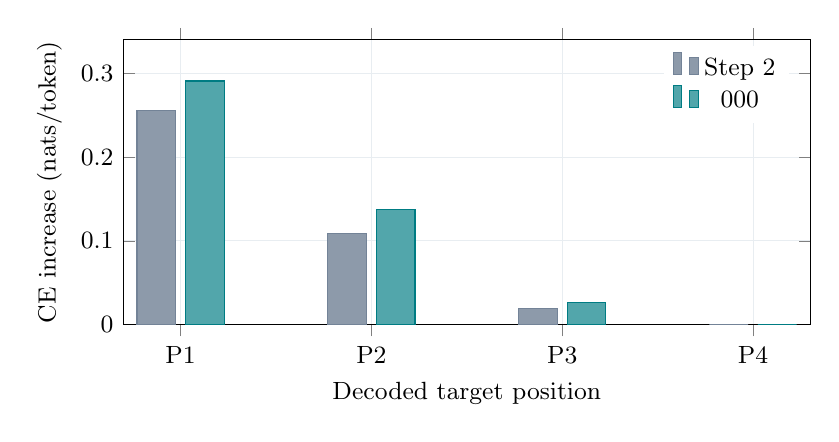
\begin{tikzpicture}
\begin{axis}[ybar=3.5pt,bar width=14pt,width=0.85\linewidth,height=5.2cm,
 ymin=0,ymax=0.34,symbolic x coords={P1,P2,P3,P4},xtick=data,
 ylabel={CE increase (nats/token)},xlabel={Decoded target position},
 legend style={draw=none,at={(0.97,0.98)},anchor=north east,font=\small},
 grid=major,grid style={linegray!60},tick label style={font=\small},label style={font=\small}]
\addplot[fill=bluegray!65,draw=bluegray!80] coordinates {(P1,0.2560)(P2,0.1085)(P3,0.0193)(P4,0)};
\addplot[fill=teal!68,draw=teal] coordinates {(P1,0.2908)(P2,0.1374)(P3,0.0260)(P4,0)};
\legend{Step 2,000,Step 2,500}
\end{axis}
\end{tikzpicture}
\caption{Sensitivity to future PLAN slots persists and grows at P1--P3 in this observed interval. The number of remaining future slots and the number of real preceding tokens both change with the target position.}
\label{fig:future}
\end{figure}

A useful interpretation of the P1 step-2,500 result is that neutralizing P2--P4 raises the average correct-token NLL by 0.2908 nats, corresponding to a factor $e^{0.2908}\simeq1.34$ in geometric-mean assigned probability for the correct token in the \emph{intact versus masked frozen model}. This is \emph{not} an estimate of the benefit over a separately trained future-free architecture.

\subsection{The persistent earlier soft proposal matters after commitment}
At P2 in the step-2,000 run, comparing the own-only and past-plus-current conditions gives
\begin{equation}
 \CE_{\mathrm{P2,own}}-\CE_{\mathrm{P2,past+current}}=0.5785-0.1085=\boxed{0.4700}\ \text{nats/token}.
 \label{eq:p2}
\end{equation}
Here the actual token $y_1$ is present through DEC2 in \emph{both} conditions; the extra input in the latter is PLAN1. This suggests a potentially useful dual representation: the decoder can consult both the original soft belief about position one and the hard identity of the token subsequently chosen.

This finding has two important limits. First, $p_1E$ is a compact expectation rather than a lossless probability vector. Second, neutralizing PLAN1 also changes the contextualized representations of other PLAN positions because those positions attend to one another bidirectionally; the observed CE difference cannot be attributed uniquely to DEC2 directly reading PLAN1 or to the uncertainty of rejected token alternatives. A soft-versus-hard replacement test and a matched retraining control would be needed to isolate those mechanisms.

\subsection{Free-running generation: predictive CE and fluency diverge}
The evaluation suite generated 64 new tokens per case using two fixed prompts (\code{math\_general\_short} and \code{science\_fluids\_short}), one seed, greedy and top-$k$ sampling ($k=40$, temperature 0.8 for sampled output). The step-2,500 outputs remained weak: invented identifiers, incomplete English, domain drift toward code, and self-repetition. For the original $S=4$ generator, greedy eight-token repetition rates were 0.0526 (math) and 0.1053 (science), while top-$k$ samples were lexically diverse but often unintelligible.

\noindent\textit{Illustrative excerpt, $S=4$ at expanded step 2,500 (math greedy):}
\begin{quote}\small\ttfamily
used to the testing of the laborator.\\
The code is a laborator, the `scape` function,\\
the `scul` function ...
\end{quote}
This sample does not demonstrate coherent mathematical explanation. Validation CE under teacher forcing must not be equated with generation quality. The small 2,048-token vocabulary and very limited parameter budget complicate broad-domain generation; a cached-generation parity audit and matched AR samples are necessary to separate representational quality from inference implementation effects.

\section{Receding-horizon experiment: commitment stride}
\subsection{Hypothesis}
Since later PLAN positions help P1, a plausible modification is to rebuild the entire $K$-position plan after every committed token and always decode from DEC1. To test this without retraining, patch 0080P4 introduced a configurable \emph{commit stride} $S\in\{1,2,4\}$ with $K=4$:
\begin{itemize}
\item $S=4$: original architecture; one PLAN prefill, four sequential DEC commitments, same plan retained.
\item $S=2$: two DEC commitments, append both real tokens to the main causal KV state, then rebuild the plan.
\item $S=1$: use DEC1 only, append its real committed token, and replan every time.
\end{itemize}
The \emph{entire} four-horizon proposal is calculated at every replan; unused positions are not accepted. Previous small-decoder PLAN state is discarded at each replan, although committed tokens remain in the main Transformer context. Hence the experiment changes both plan freshness and plan persistence and cannot attribute an outcome uniquely to one of them.

\subsection{Paired causal-inference scoring and work}
For each stride, a correctness-first generator uses the original causal main-model cache, precomputes all PLAN keys/values, and appends only true earlier tokens when scoring reference continuations. Eight fixed held-out rows with up to 32 targets each yielded exactly 256 scored tokens in this run. The measured losses are \emph{causal-inference-procedure CE}, not identical to the earlier full-window 0080K training validation.

\begin{table}[ht]
\centering
\caption{Frozen step-2,500 commitment-stride comparison on 256 paired reference targets. Work counts are proposal PLAN prefills, not a measurement of full GPU inference FLOPs or latency.}
\label{tab:stride}
\begin{tabular}{@{}lrrrr@{}}\toprule
Stride & CE (nats/token) & $\Delta$ CE vs $S=4$ & Full plans & Plans/token\\\midrule
$S=4$ & \textbf{3.96349} & 0 & 64 & 0.250\\
$S=2$ & 4.02332 & +0.05983 & 128 & 0.500\\
$S=1$ & 4.02431 & +0.06082 & 256 & 1.000\\\bottomrule
\end{tabular}
\end{table}

\begin{figure}[ht]
\centering
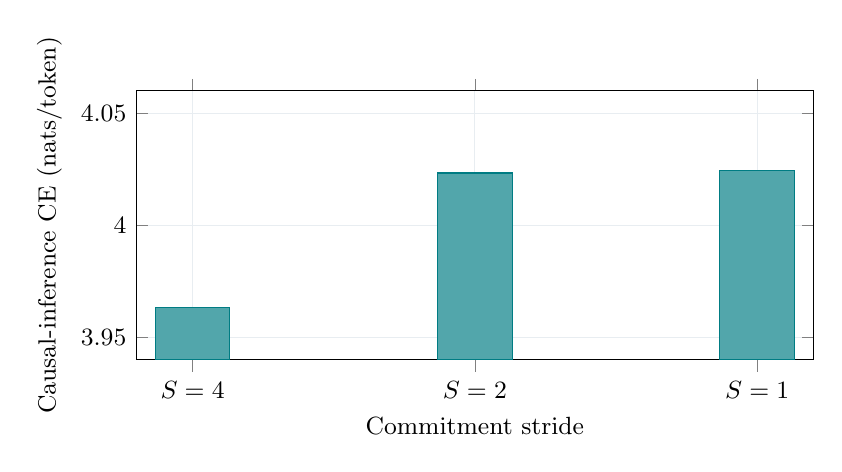
\begin{tikzpicture}
\begin{axis}[width=.84\linewidth,height=5.0cm,symbolic x coords={S4,S2,S1},xtick=data,
 xticklabels={$S=4$,$S=2$,$S=1$},ymin=3.94,ymax=4.06,
 ylabel={Causal-inference CE (nats/token)},xlabel={Commitment stride},
 ybar,bar width=27pt,grid=major,grid style={linegray!60},tick label style={font=\small},label style={font=\small}]
\addplot[fill=teal!68,draw=teal] coordinates {(S4,3.96349)(S2,4.02332)(S1,4.02431)};
\end{axis}
\end{tikzpicture}
\caption{The original $S=4$ model scores best on this small paired sample, despite performing fewer proposal prefills. The axis is truncated to resolve the observed differences.}
\label{fig:stride}
\end{figure}

\subsection{Interpretation and free-running comparison}
The frozen model trained with complete four-token blocks scored better when it retained its original plan for all four DEC decisions. Replanning every token incurred roughly four times as many full-plan evaluations, with $\approx0.061$ nats/token higher CE on this small sample. The most plausible confounds are: (i) $S=1$ repeatedly invokes DEC1 in contexts offset from the trained block grid; (ii) replan-and-discard removes earlier soft-plan information that was demonstrably useful to later DEC positions; and (iii) fresh main-model conditioning may not compensate for losing learned causal DEC interactions. A stride-aware retrained model could behave differently.

Free-running text does \emph{not} show a corresponding clear quality ranking. For example, the two greedy $S=1$ generations had lower exact eight-gram repetition (0.0175 for math, 0.0000 for science) than the $S=4$ samples (0.0526 and 0.1053), yet both retained obvious semantic repetition, invented words, and poor relevance to the prompts. Thus fewer repeated eight-grams are not evidence of better overall language quality. Only two prompts and one seed were evaluated; these generation metrics are exploratory.

\section{What is established, what is not, and next experiments}
\subsection{Supported findings}
\begin{enumerate}
\item A $K=4$ model with a small dense prefix decoder can be trained end-to-end on packed, document-aware real text with the intended causal block alignment.
\item The correct soft PLAN representations affect held-out teacher-forced predictions even with the same direct proposal-logit prior and shifted ground-truth DEC prefix.
\item A PLAN for a later future position affects earlier decisions, especially P1, whose within-block committed prefix is empty.
\item Earlier soft PLAN slots remain useful to the frozen model after corresponding ground-truth tokens enter its causal DEC prefix.
\item For the \emph{existing $S=4$-trained checkpoint}, inference-only frequent replanning did not improve paired held-out causal CE, despite increasing proposal computations.
\end{enumerate}

\subsection{Open questions and threats to validity}
\begin{enumerate}
\item \textbf{Distribution-shifted ablations:} neutral embeddings are outside the trained plan distribution. Context-shuffled realistic proposals, hard-committed-token substitutions, attention tracing, and separately retrained controls are necessary.
\item \textbf{Teacher forcing:} later final CE benefits from true preceding tokens, whereas free-running decoding accumulates its own errors. The recorded generation samples remain weak.
\item \textbf{No matched AR or multi-token comparison:} superiority over a conventional AR model, comparable auxiliary multi-horizon heads, or a parameter/FLOP-matched prefix decoder is not established.
\item \textbf{Small and partly heterogeneous evaluations:} the stride evaluation uses only 256 targets, while other tests use a separate fixed validation regimen. Need document-clustered confidence intervals and more contexts/seeds.
\item \textbf{Information content:} a soft expectation $pE$ does not preserve the entire vocabulary distribution. A measured loss penalty does not prove an explicit sequence-level latent variable, semantic planning, or a new $V^K$ discrete vocabulary.
\item \textbf{Scale and implementation:} the CPU experiment does not verify 500M quality or RTX 5080 throughput. Full routed long-context cached generation, objective parity, device peak memory and actual runtime require separate tests.
\item \textbf{Long-range effects:} short-block consistency does not automatically solve repetitions or topic drift across many blocks.
\end{enumerate}

\subsection{Proposed next experiments}
\begin{enumerate}
\item \term{Matched autoregressive baseline:} same tokenizer, corpus, number of distinct supervised target tokens, held-out documents, backbone parameter and compute budgets, plus separately controlled inference time.
\item \term{Realistic future-plan permutation:} retain P1 but substitute P2--P4 soft vectors from unrelated held-out contexts; examine P1 CE under document-level repeated seeds. Keep residual logits and committed tokens fixed.
\item \term{Past soft versus committed hard:} at P2 compare original $p_1E$, the committed embedding $E[y_1]$, a shuffled soft $p_1'E$, and a neutral expectation, keeping the true hard prefix constant; retrain corresponding decoders to address OOD artifacts.
\item \term{Horizon and decoder-size sweeps:} $K=2,4,8$ and several small decoder capacities with matched target-token counts, seeds and effective compute; plot per-horizon CE and loss penalties at comparable stages.
\item \term{Stronger stride evaluation:} evaluate many more held-out documents, inspect original-block-position CE and cache parity, then test a stride-aware trained model if evidence warrants the cost.
\item \term{Free-running robustness:} longer prompt suites, grammar/coherence judgments, repetition onset, semantic repetition, domain adherence, greedy and sampling, and error analysis at $K$ boundaries.
\item \term{Scaled implementation audit:} on a separate $\sim$500M backbone, first establish numerical/causal parity, then train and benchmark memory, supervised tok/s, prefill, cached decode, and wall-clock cost.
\end{enumerate}

\section{Conclusion}
The 0080 architecture is best understood as a \emph{persistent continuous plan conditioned on causal context, resolved by a separate causal commitment stream}. Rather than converting four future marginals into a fixed set of independent token decisions, the decoder retains the original soft predictions throughout the block, jointly contextualizes those predictions with bidirectional PLAN attention, and performs sequential commitments that can consult both previous hard tokens and previous soft beliefs.

Initial 7M-class results show measurable, sometimes growing sensitivity to the complete PLAN pathway and strong first-position dependence on future proposals. These observations motivate investigation of local sequence-level representation, but do \emph{not} yet establish semantic planning, improved generation coherence, or better efficiency than matched existing techniques. The negative frozen commitment-stride experiment is useful: it cautions that repeatedly recomputing the horizon is not automatically preferable to retaining a coherent, shared uncertainty representation. The next stage is discriminating ablation and matched-baseline science, followed by scale-sensitive evaluation.

\appendix
\section{Source-code map and reproducibility commands}
The following repository paths describe the experimental design. They are implementation references, not a guarantee that every development branch contains identical files. The report is intended to be committed under a directory such as \path{docs/research/}.
\begin{itemize}
\item \path{mini_llm/block_proposal/proposals.py}: shared nonlinear horizon proposal head.
\item \path{mini_llm/block_proposal/decoder.py}: soft expectation projection, prefix Transformer, residual correction, manual gradients.
\item \path{mini_llm/block_proposal/contracts.py}: causal block schedule, shifted DEC targets and prefix mask.
\item \path{mini_llm/block_proposal/training.py}: one-trunk forward/backward, bounded independent-block groups.
\item \path{mini_llm/block_proposal/generation.py}: cached soft PLAN prefix and sequential commitment; stride $S$.
\item \path{examples/train_block_proposal_cpu_learning_0080i.py}: CPU experiment, warm-start and strict resume lineage.
\item \path{examples/evaluate_block_proposal_cross_position_0080k.py}: frozen horizon-specific PLAN controls.
\item \path{examples/evaluate_block_proposal_stride_0080p4.py}: paired causal-inference CE for strides.
\item \path{benchmarks/evaluate_generation.py}: two-prompt, multi-strategy free-running benchmark.
\end{itemize}

\subsection{PowerShell: fixed cross-position ablation}
\begin{lstlisting}[language={},caption={Run against step 2,500 of the expanded-data experiment; from repository root.}]
$env:MINI_LLM_BACKEND = "numpy"
$env:OPENBLAS_NUM_THREADS = "8"
$env:OMP_NUM_THREADS = "8"
.\.venv\Scripts\python.exe -m examples.evaluate_block_proposal_cross_position_0080k `
  --mixed-shard-root .\data\block_proposal_cpu_two_sources_50k `
  --training-output .\benchmarks\results\0080p2_cpu_50k_warmstart `
  --checkpoint .\benchmarks\results\0080p2_cpu_50k_warmstart\checkpoints\two_stage\step_00002500 `
  --output .\benchmarks\results\0080p2_cpu_50k_warmstart\cross_position_step_00002500.json
\end{lstlisting}

\subsection{PowerShell: paired commitment-stride evaluation}
\begin{lstlisting}[language={},caption={The reported small-sample $S\in\{4,2,1\}$ likelihood sweep.}]
.\.venv\Scripts\python.exe -m examples.evaluate_block_proposal_stride_0080p4 `
  --mixed-shard-root .\data\block_proposal_cpu_two_sources_50k `
  --training-output .\benchmarks\results\0080p2_cpu_50k_warmstart `
  --checkpoint .\benchmarks\results\0080p2_cpu_50k_warmstart\checkpoints\two_stage\step_00002500 `
  --strides 4,2,1 `
  --validation-rows 8 `
  --target-tokens 32 `
  --output .\benchmarks\results\0080p2_cpu_50k_warmstart\stride_2500_rows8_t32.json
\end{lstlisting}

\subsection{PowerShell: qualitative generation by stride}
\begin{lstlisting}[language={},caption={Same frozen checkpoint and prompts for all three strides.}]
foreach ($stride in @(4, 2, 1)) {
  .\.venv\Scripts\python.exe -m benchmarks.evaluate_generation `
    --architecture block-proposal-0080i `
    --checkpoint ".\benchmarks\results\0080p2_cpu_50k_warmstart\checkpoints\two_stage\step_00002500" `
    --tokenizer-path ".\data\block_proposal_cpu_two_sources\tokenizer.json" `
    --commit-stride $stride `
    --output-dir ".\benchmarks\results\0080p4_generation_s${stride}_2500" `
    --prompt-ids "math_general_short,science_fluids_short" `
    --seeds 42 --strategies "greedy,top-k" `
    --top-k 40 --temperature 0.8 --max-new-tokens 64 `
    --print-generations
}
\end{lstlisting}

\subsection{Run provenance and data availability}
The figures and tables were transcribed from user-reported console output for the specific local checkpoints. They were not independently recomputed against the original locally trained checkpoint files in the report-authoring environment. To fully reproduce, preserve checkpoint directories, tokenizers, packed-shard manifests, fixed validation JSONL, experiment output JSON, and generation JSONL. Actual document counts, valid-token totals and hardware timing should be exported from immutable run manifests in a future revision. Do not overwrite the original 5,000-step restricted-corpus run when repeating expanded-data experiments.

\section{Earlier restricted-corpus K=4 result (not matched)}
\begin{table}[ht]
\centering
\caption{Original restricted-corpus step-5,000 horizon losses, included only for historical context. This used a different prepared dataset and validation draw; do not compare the absolute values directly against the expanded-corpus tables.}
\begin{tabular}{@{}lrrr@{}}\toprule
Horizon & Proposal CE & Final CE & Gain\\\midrule
P1 & 4.9904 & 4.5834 & +0.4070\\
P2 & 6.0034 & 4.5850 & +1.4184\\
P3 & 6.3900 & 4.6409 & +1.7491\\
P4 & 6.4153 & 4.4510 & +1.9644\\\bottomrule
\end{tabular}
\end{table}
The results initially motivated investigation of cross-position representations, but the strong later-position decoder gains are also naturally influenced by teacher-forced earlier tokens. Historical K=8 experiments used different schedules/data and cannot establish the best $K$.

\begin{thebibliography}{9}
\bibitem{vaswani2017} A. Vaswani et al., \emph{Attention Is All You Need}, Advances in Neural Information Processing Systems, 2017. \url{https://arxiv.org/abs/1706.03762}.
\bibitem{dong2019} L. Dong et al., \emph{Unified Language Model Pre-training for Natural Language Understanding and Generation}, Advances in Neural Information Processing Systems, 2019. \url{https://arxiv.org/abs/1905.03197}.
\bibitem{gloeckle2024} F. Gloeckle, B. Youbi Idrissi, B. Rozi\`ere, D. Lopez-Paz, and G. Synnaeve, \emph{Better \& Faster Large Language Models via Multi-token Prediction}, 2024. \url{https://arxiv.org/abs/2404.19737}.
\bibitem{cai2024} T. Cai et al., \emph{Medusa: Simple LLM Inference Acceleration Framework with Multiple Decoding Heads}, Proceedings of ICML, 2024. \url{https://proceedings.mlr.press/v235/cai24b.html}.
\end{thebibliography}
\end{document}
